El término cienciometría fue definido por primera vez por Nalimov, en 1971, mientras desarrollaba ``los métodos cuantitativos para la investigación y desarrollo de la ciencia como un proceso de información'' \cite{nalimov1971measurement}. 

Luego el término fue mutando y refinándose hasta llegar a la definición más moderna y amplia, como la que utiliza Hess \cite{hess1997science} al afirmar que la cienciometría es el ``estudio cuantitativo de la ciencia, la comunicación de la ciencia y la política científica''. 

Planteada inicialmente como un conjunto de mediciones empíricas sobre la producción científica, la disciplina viró rápidamente hacia un análisis mucho más profundo y con implicancias en todas las facetas de la ciencia, la educación y la toma de decisiones sobre políticas del ecosistema científico a nivel mundial, ocupando un lugar de importancia en la triada conformada además por las ciencias de la información y la sociología de la ciencia (ver Figura \ref{fig:ambito-cienciometria}\cite{munoz2017analisis}).

En poco tiempo los indicadores cienciométricos comenzaron a complementar la toma de decisiones en organizaciones para la implementación de políticas científicas, tales como la Oficina Nacional de las Ciencias (National Science Board) de Estados Unidos, que en 1972 inicia la publicación bianual de \textit{Indicadores Científicos (Science Indicators)}.

\begin{figure}[H]
	\centering
	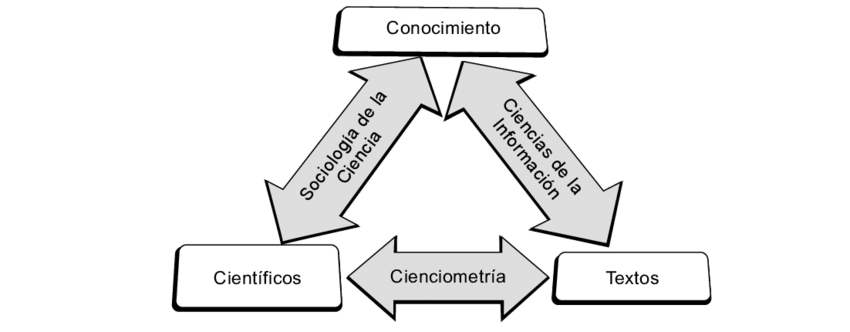
\includegraphics[width=0.9\linewidth]{images/ambito-cienciometria}
	\caption{\textbf{Ámbito de aplicación de la cienciometría}} 
	\label{fig:ambito-cienciometria}
\end{figure}

El estudio comparativo de la producción científica, tanto a nivel personal como institucional, e incluso regional y mundial viene demostrando ser una herramienta eficaz para la caracterización de los avances en las distintas ramas de las ciencias a la vez que brinda herramientas para la toma de decisiones basadas en evidencia contrastable \cite{vinkler2008correlation,munoz2017analisis}. 

La posibilidad de tener una visión dinámica de los cambios producidos en las distintas ramas científicas resulta hoy de fundamental importancia para poder observar los resultados e impacto producto de la aplicación de las distintas medidas tomadas con respecto a política científica, de investigación y desarrollo, y educativa.

\subsection{El objeto de estudio}

El principal objeto de estudio de la cienciometría son los artefactos que se producen como resultado del proceso de investigación \cite{chen2002mapping}. Estos artefactos toman la forma de publicaciones, que pueden diferir entre sí en el medio utilizado, la periodicidad, el tipo, etc. pero que siempre cuentan con algunas características comunes.

Los artefactos utilizados, en los análisis cienciométricos, cuentan con atributos tales como:

\begin{itemize}
	\item Titulo
	\item Autor o autores
	\item Contenido
	\item Referencias
	\item Ámbito de estudios
	\item Medio utilizado para su publicación
	\item Publicación que contiene el trabajo
	\item Fecha o año de publicación
\end{itemize}
